\documentclass[10pt, a5paper]{article}
\usepackage{pdfpages}
\usepackage{parallel}
\usepackage[T2A]{fontenc}
\usepackage{ucs}
\usepackage[utf8x]{inputenc}
\usepackage[polish,english,russian]{babel}
\usepackage{hyperref}
\usepackage{rotating}
\usepackage[inner=2cm,top=1.8cm,outer=2cm,bottom=2.3cm,nohead]{geometry}
\usepackage{listings}
\usepackage{graphicx}
\usepackage{wrapfig}
\usepackage{longtable}
\usepackage{indentfirst}
\usepackage{array}
\newcolumntype{P}[1]{>{\raggedright\arraybackslash}p{#1}}
\frenchspacing
\usepackage{fixltx2e} %text sub- and superscripts
\usepackage{icomma} % коскі ў матэматычным рэжыме
\PreloadUnicodePage{4}

\newcommand{\longpage}{\enlargethispage{\baselineskip}}
\newcommand{\shortpage}{\enlargethispage{-\baselineskip}}

\def\switchlang#1{\expandafter\csname switchlang#1\endcsname}
\def\switchlangbe{
\let\saverefname=\refname%
\def\refname{Літаратура}%
\def\figurename{Іл.}%
}
\def\switchlangen{
\let\saverefname=\refname%
\def\refname{References}%
\def\figurename{Fig.}%
}
\def\switchlangru{
\let\saverefname=\refname%
\let\savefigurename=\figurename%
\def\refname{Литература}%
\def\figurename{Рис.}%
}

\hyphenation{admi-ni-stra-tive}
\hyphenation{ex-pe-ri-ence}
\hyphenation{fle-xi-bi-li-ty}
\hyphenation{Py-thon}
\hyphenation{ma-the-ma-ti-cal}
\hyphenation{re-ported}
\hyphenation{imp-le-menta-tions}
\hyphenation{pro-vides}
\hyphenation{en-gi-neering}
\hyphenation{com-pa-ti-bi-li-ty}
\hyphenation{im-pos-sible}
\hyphenation{desk-top}
\hyphenation{elec-tro-nic}
\hyphenation{com-pa-ny}
\hyphenation{de-ve-lop-ment}
\hyphenation{de-ve-loping}
\hyphenation{de-ve-lop}
\hyphenation{da-ta-ba-se}
\hyphenation{plat-forms}
\hyphenation{or-ga-ni-za-tion}
\hyphenation{pro-gramming}
\hyphenation{in-stru-ments}
\hyphenation{Li-nux}
\hyphenation{sour-ce}
\hyphenation{en-vi-ron-ment}
\hyphenation{Te-le-pathy}
\hyphenation{Li-nux-ov-ka}
\hyphenation{Open-BSD}
\hyphenation{Free-BSD}
\hyphenation{men-ti-on-ed}
\hyphenation{app-li-ca-tion}

\def\progref!#1!{\texttt{#1}}
\renewcommand{\arraystretch}{2} %Іначай формулы ў матрыцы зліпаюцца з лініямі
\usepackage{array}

\def\interview #1 (#2), #3, #4, #5\par{

\section[#1, #3, #4]{#1 -- #3, #4}
\def\qname{LVEE}
\def\aname{#1}
\def\q ##1\par{{\noindent \bf \qname: ##1 }\par}
\def\a{{\noindent \bf \aname: } \def\qname{L}\def\aname{#2}}
}

\def\interview* #1 (#2), #3, #4, #5\par{

\section*{#1\\{\small\rm #3, #4. #5}}

\def\qname{LVEE}
\def\aname{#1}
\def\q ##1\par{{\noindent \bf \qname: ##1 }\par}
\def\a{{\noindent \bf \aname: } \def\qname{L}\def\aname{#2}}
}

\begin{document}
\title{Безупречная история в Git или Mercurial}
\author{Алексей Хлебников, Осло, Норвегия\footnote{\url{alexei.khlebnikov@gmail.com}, \url{http://lvee.org/en/abstracts/125}}}
\maketitle
\begin{abstract}
History of development saved in version control systems (VCS) is very important. It simplifies investigation of problems, reversi\-on of regressions, picking specific changes for specific customers or releases, learning code for new developers in a team, generally keeping control over the code, assigning blame, etc. However, after long development of a complex software product, its VCS history is often hard to read. The talk shows  ways to remedy the problem by consistent use of branching, rebasing and squashing, with detailed examples for Git and Mercurial.
\end{abstract}
\subsection*{Введение}

Существуют различные способы использования VCS в процессе разработки. Некоторые команды просто коммитят всё в основную ветку одного репозитория. Иные используют ветвление (branching), слияние (merging), несколько репозиториев (cloning). Ниже предлагается вариант, который удобен разработчикам и в то же время оптимизирован для улучшения читаемости истории VCS. Иными словами, как правильно бранчить, сквошить и ребэйсить код, используя команды Git и Mercurial.

\subsection*{Важные приёмы процесса разработки}

\subsubsection*{Ветвление (branching)}

Ветвление имеет следующие преимущества:

\begin{itemize}
  \item Работая в отдельной ветке над отдельным кейсом (case), вы можете свободно экспериментировать, не боясь сломать main"=line. Это важно не только технически, но и психологически: над разработчиком не довлеет груз ответственности и он может позволить себе большую свободу действий.
  \item Соответственно, коммиты других участников проекта на других ветках не смогут ничего сломать на вашей собственной ветке.
  \item Все коммиты, относящиеся к данному кейсу, сгруппированы. Они идут по порядку, в отличие от ситуации, когда все участники разработки используют только одну ветку. Это облегчает понимание кода данного кейса и улучшает историю в VCS.
  \item Пока код данной ветки не доставлен в mainline, можно редактировать историю (остановимся на этом позже).
\end{itemize}

Без ветвления все коммиты идут вперемешку на mainline:
\begin{figure}[h!]
  \centering
  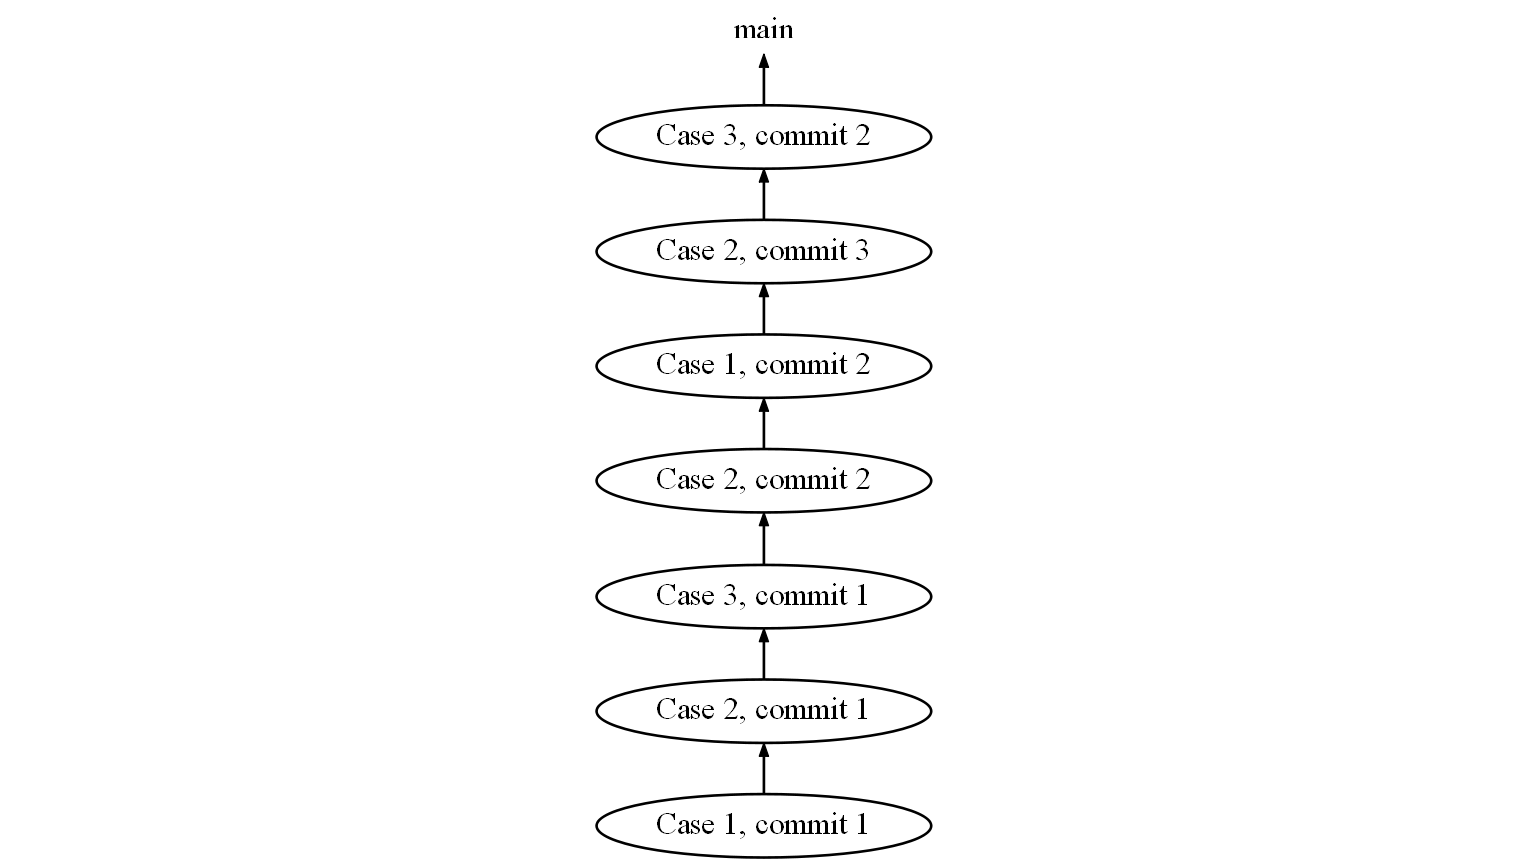
\includegraphics[scale=0.2]{02_2014_only-main.png}
\end{figure}

При ветвлении коммиты группируются по кейсам:
\begin{figure}[h!]
  \centering
  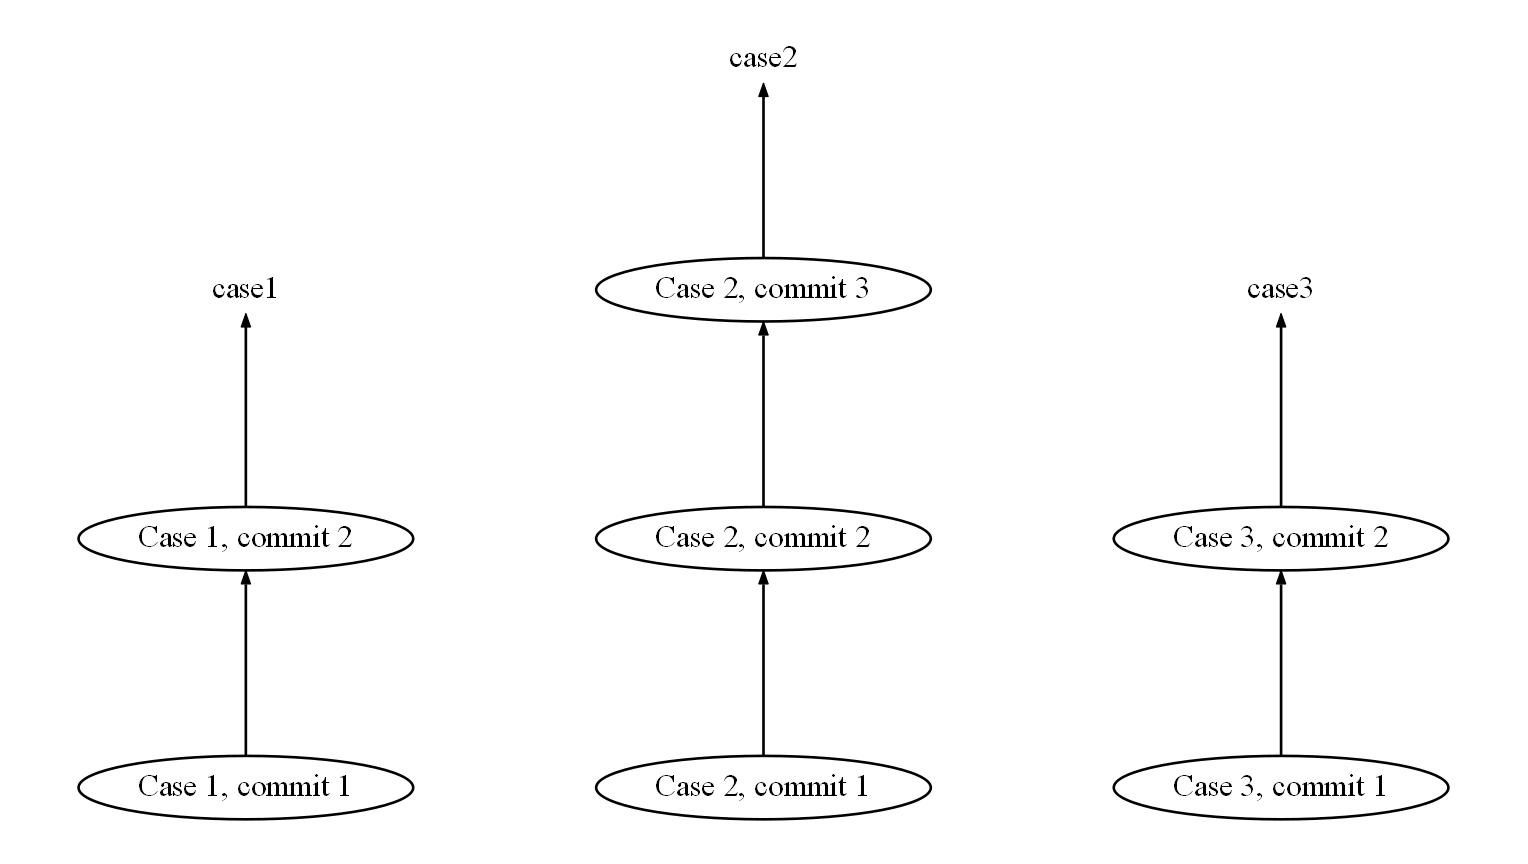
\includegraphics[scale=0.2]{02_2014_branches.png}
\end{figure}

\subsubsection*{Rebasing}

Rebasing может применяться в процессе работы над кейсом, а также для доставки коммитов в mainline.

Rebasing в процессе работы позволяет:

\begin{itemize}
  \item Получить ответвление от обновлённого mainline.
  \item Разрешать merge-conflicts небольшими порциями в ходе работы, а не одним большим куском в самом конце.
  \item Тестировать код своего кейса относительно нового mainline без его доставки в этот самый mainline.
\end{itemize}

Rebase вместо Merge как метод доставки кода в mainline позволяет получить:

\begin{itemize}
  \item Линейную историю в VCS. Линия проще и наглядней графа.
  \item Меньше проблем с blame, bisect и revert. Эти команды работают лучше на коммитах с одним родителем, чем с несколькими.
  \item Возможность удалять очень старые ветки (и их коммиты) из репозитория. Это повышает быстродействие репозитория. А если эти ветки всё-таки нужны "--- их можно хранить в архивном репозитории или в бэкапе. Тем, кто считает замедление репозитория при увеличении количества коммитов надуманной проблемой, есть смысл ознакомиться с исследованием Facebook \cite{Hlebnikov1}.
\end{itemize}

При доставке кода в mainline через Merge, mainline состоит в основном из merge-коммитов:
\begin{figure}[h!]
  \centering
  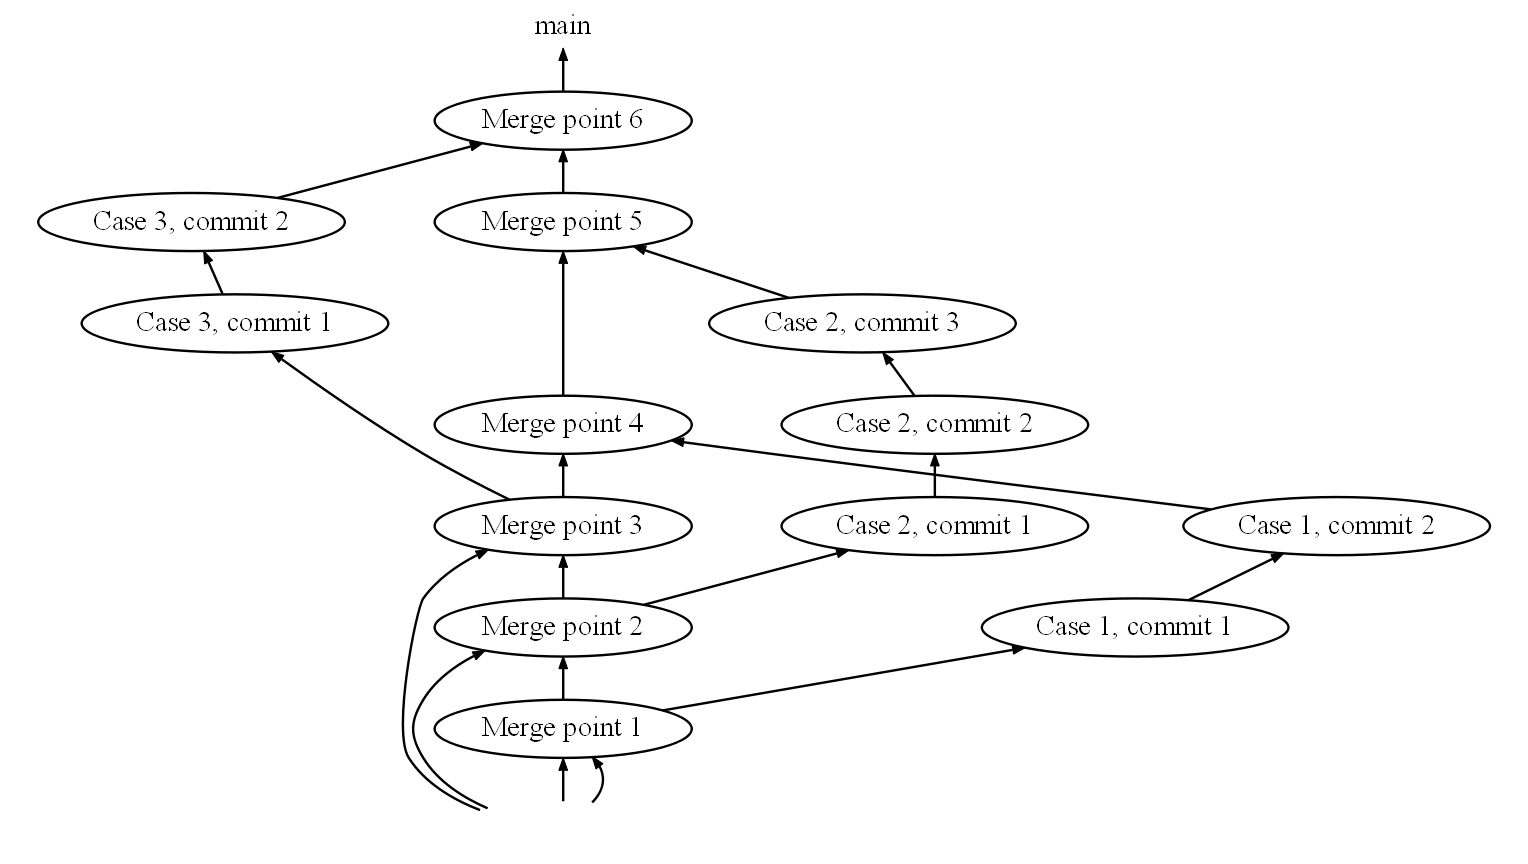
\includegraphics[scale=0.2]{02_2014_main-merged.png}
\end{figure}

Тот же самый граф, но без ярко выраженного вертикального mainline:
\begin{figure}[h!]
  \centering
  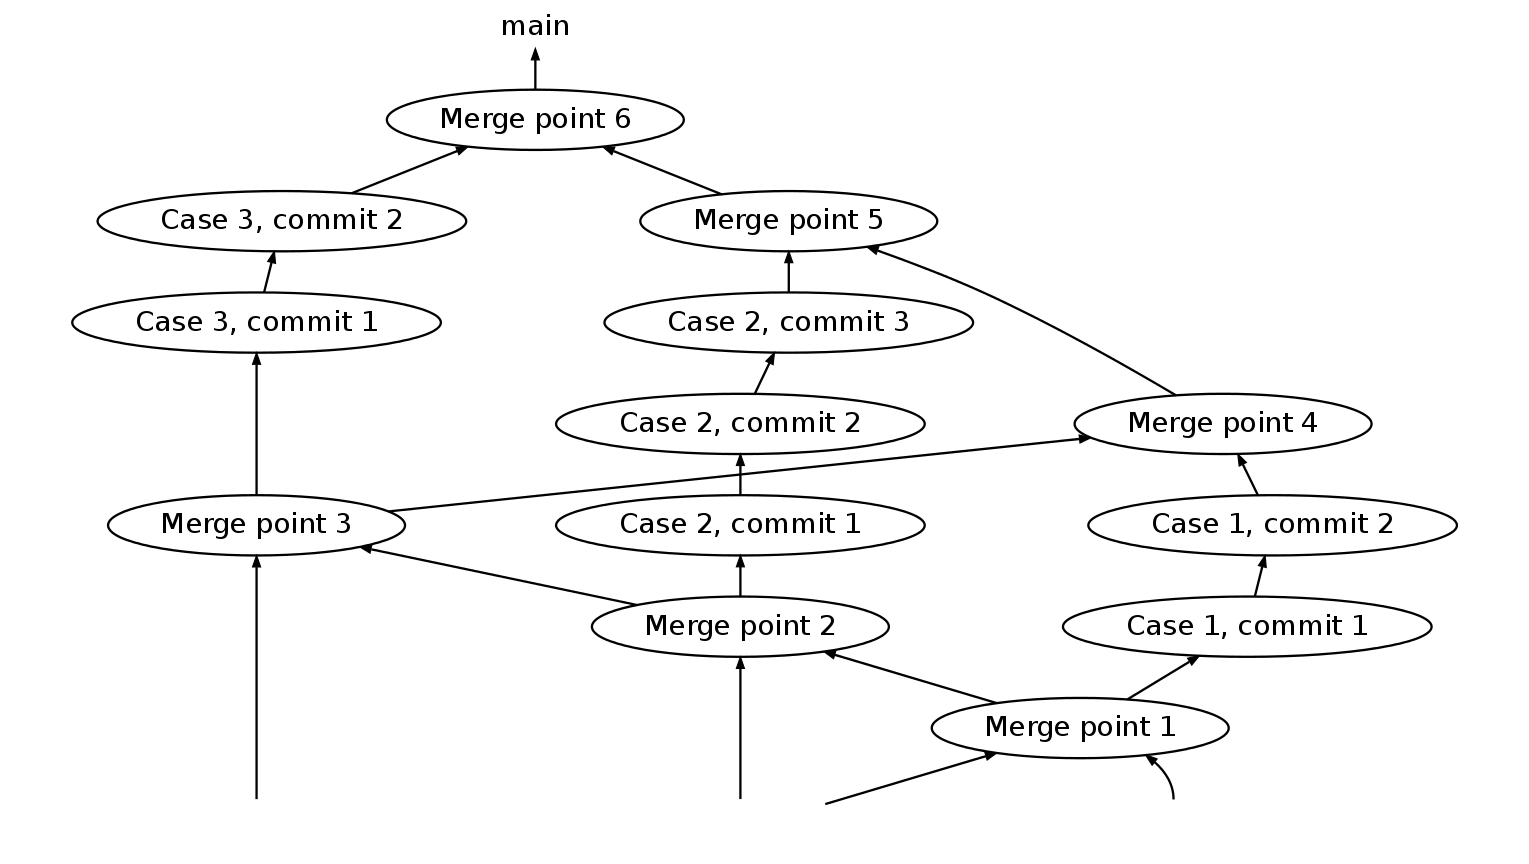
\includegraphics[scale=0.2]{02_2014_main-merged-weak-mainline.png}
\end{figure}

Как видно, в такой истории довольно трудно разобраться, особенно по прошествии долгого времени, или если разбирающийся "--- новый человек на проекте. В этом графе даже mainline трудно найти.

А вот история, которая получается при Rebase:
\begin{figure}[h!]
  \centering
  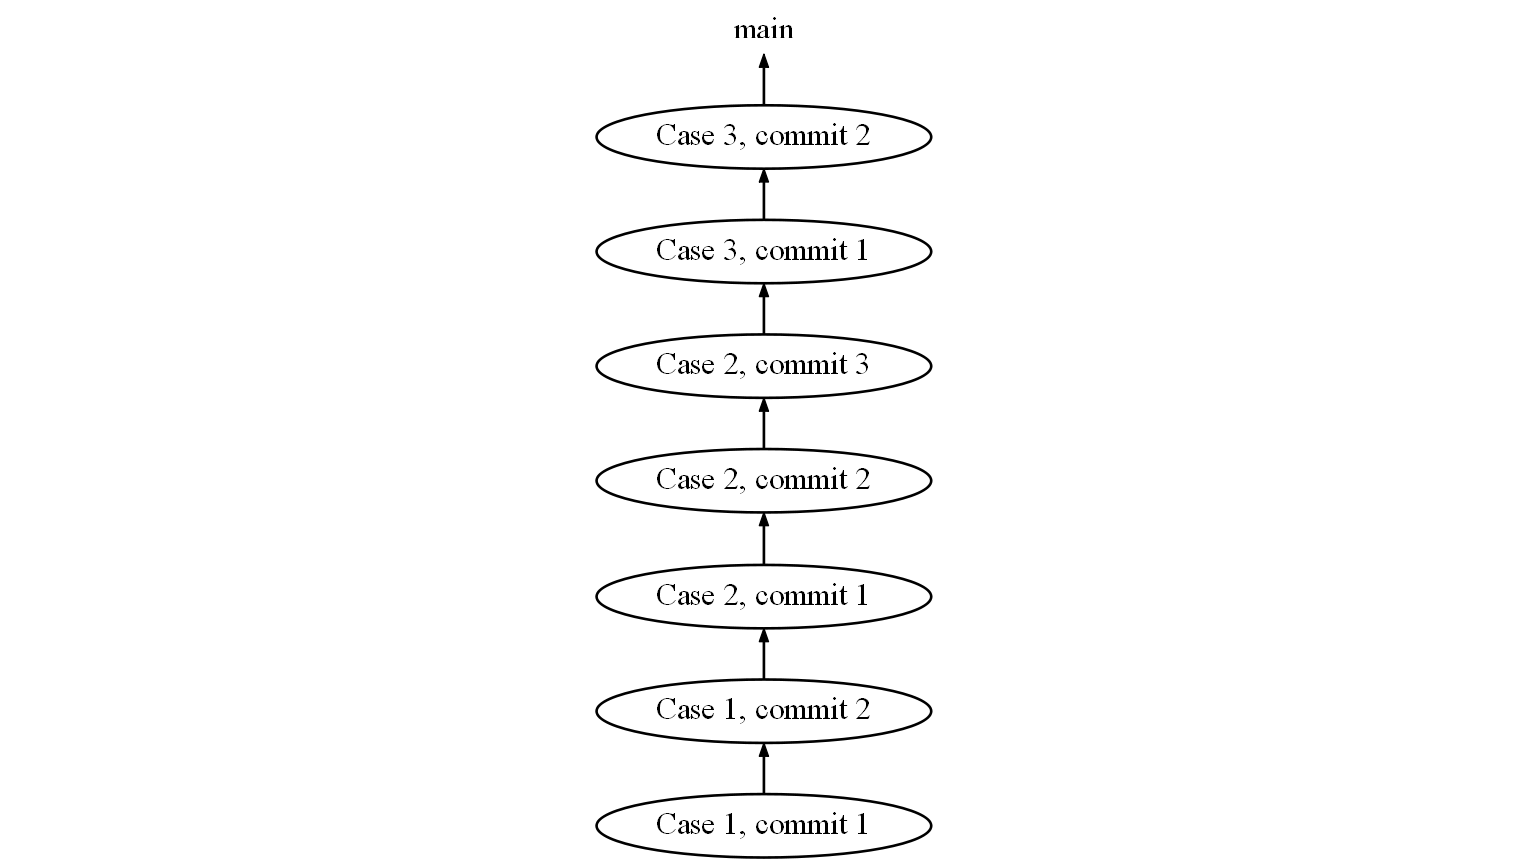
\includegraphics[scale=0.2]{02_2014_main-ordered.png}
\end{figure}

Как видно, история линейна, что сильно улучшает её читаемость. Но можно сделать ещё лучше "--- уменьшить количество коммитов. И в этом поможет squashing.

\subsubsection*{Squashing}

Squashing "--- это слияние нескольких коммитов в один. Squashing позволяет получить:

\begin{itemize}
  \item Компактную историю. Это тем важнее, чем дольше идёт разработка и чем больше коммитов собралось в репозитории.
  \item Меньше мусора в истории.
  \item Более лёгкий откат изменений.
\end{itemize}

Если после работы над кейсом ветка содержит много мусора в истории\ldots{}
\begin{figure}[h!]
  \centering
  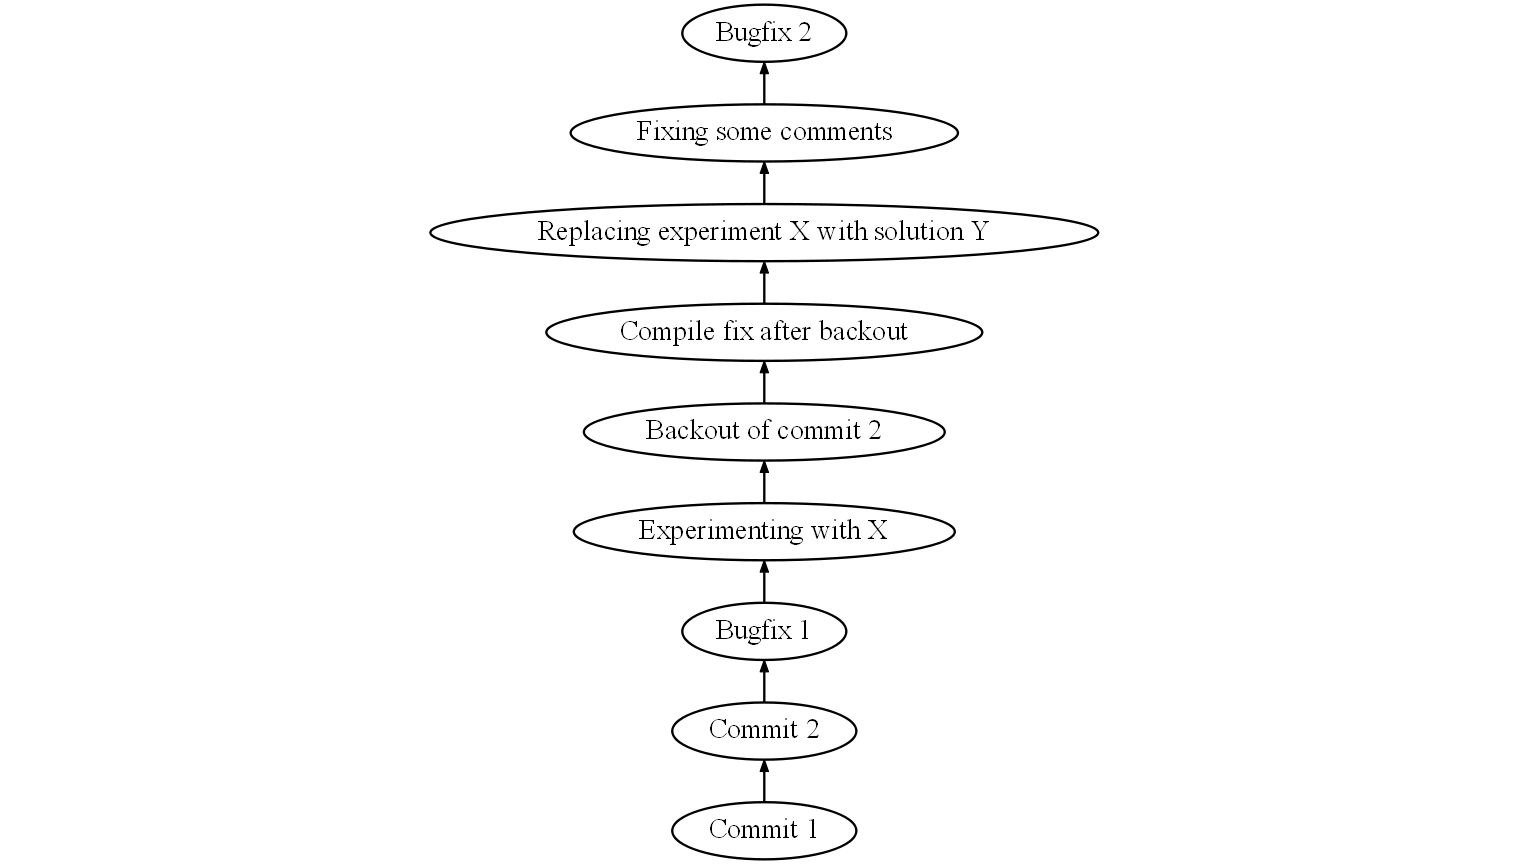
\includegraphics[scale=0.2]{02_2014_history-with-garbage.png}
\end{figure}

\ldots{}squashing позволит избавиться от этого мусора, слив все комиты в один:
\begin{figure}[h!]
  \centering
  
\includegraphics[scale=0.3]{02_2014_history-without-garbage.png}
\end{figure}

\subsection*{Конкретные команды, шаг за шагом}

Приведем примеры команд для Git и Mercurial в виде таблицы:

\begin{table}
  \centering
  \begin{tabular}{P{2.5cm}|P{3.5cm}|P{3.5cm}}
    \hline
                                  ~  & \textbf{Git}                   & \textbf{Mercurial}          \\ \hline
    Ответвление от mainline          & git checkout -{}-b case4       & hg book case4              \\
    Работа над кейсом                & git commit -m "Commit 1" \newline
                                       git commit -m "Commit 2" \ldots{}
                                                                    & hg commit -m "Commit 1" \newline
                                                                      hg commit -m "Commit 2" \ldots{} \\
    Rebase и squash              & git checkout -{}-b \emph{case4-2} \newline
                                   git rebase -{}-interactive main
                                                     & (нужны расширения rebase и histedit) \newline
                                                       hg rebase -{}-keep -{}-dest main \newline
                                                       hg histedit main \newline
                                                       hg book \emph{case4-2}      \\
    \hline
  \end{tabular}
\end{table}
Отдельно коснёмся «табу на rebase после push». Существует довольно распространённый миф, что если ветка запушена (push) на сервер "--- все возможности ребэйса (rebase) для неё потеряны, потому что если ветку проребэйсить и запушить на сервер опять (что возможно только с ключом --force), то это создаст несоответствие между репозиторием на сервере и репозиториями других разработчиков. В результате эти разработчики при попытке подтянуть эту ветку с сервера получат сломанную ветку.

На самом деле rebase возможен, если выполнять его правильно. На примере команд, приведённых в таблице, видно, что при ребэйсинге создаётся новая ветка, \textbf{case4-2}. Это принципиальный момент. Первоначальная ветка, \textbf{case4}, так и остаётся на своём месте, и получается аналог copy-on-write. Таким образом консистентность репозитория не нарушается, и ветка case4 не ломается "--- она просто устаревает. Теперь про неё можно забыть, а дальнейшую разработку, если она ещё продолжается, вести на ветке case4-2.

Также следует обратить внимание на ключ --interactive для Git и команду histedit для Mercurial. В результате их использования Git или Mercurial вызывают текстовый редактор, в котором разработчик может редактировать историю своей ветки: помечать коммиты для правки комментария, сливать несколько коммитов вместе, менять коммиты местами, удалять ненужные коммиты.

В сущности, многие коммиты "--- просто мусор в истории VCS: неудавшиеся эксперименты, багфиксы, фиксы компиляции, чистка неиспользуемых переменных, исправления опечаток в комментариях. Подобный материал в истории VCS не представляет ровным счётом никакого интереса. Как правило, от разработчика требуется имплементация фичи X или исправление бага Y, и желательно одним куском (то есть, как правило (хоть и не всегда), одним коммитом). А детали того, через что разработчик прошёл в процессе разработки, никого не интересуют. По этой причине мелкие правящие коммиты всегда имеет смысл объединить с «главными» коммитами, которые они дополняют. Это же относится и к фиксам в результате code review.

Делать слишком много «главных» коммитов для одного кейса тоже не имеет смысла. Наоборот, для большинства кейсов перед доставкой кода в mainline лучше слить все коммиты в один и использовать название кейса как комментарий этого единственного коммита. Если имел место рефакторинг без изменения функциональности "--- его имеет смысл выделить в отдельный коммит. Если имели место фиксы багов mainline'a, которые проявились при работе над данным кейсом "--- их тоже имеет смысл выделить в отдельные коммиты, и поместить эти коммиты перед основной разработкой. Других коммитов не нужно. Это и есть squashing "--- слияние нескольких коммитов в один.

Кроме чистки мусора в истории squashing также помогает убрать коммиты, которые не компилируются, путём слияния с фиксом компиляции. Это важно, если  используется bisect, а также в случае отката изменений.

Если вам захочется оставить в истории VCS свои чаяния и веяния по поводу данного кейса из ностальгических соображений "--- есть возможность сохранить их только для себя на той старой ветке case4, которая была любезно сохранена при copy-on-write-rebase. Не перетаскивая свой мусор в mainline, разработчик заодно не создает аналогичного искушения для товарищей по команде.

\subsection*{Доставка кода в mainline}

Итак, работа над кейсом завершена, код кейса оттестирован с новейшим mainline. После финальных rebase и squash на ветке должна находиться краткая и красивая история кейса, а сама ветка основана на верхушке mainline. Это и есть подходящий момент для доставки кода кейса в mainline. Для этого надо всего лишь переместить указатель mainline вперёд по ветке case4-2 "--- сделать fast-forward. Это можно сделать несколькими способами; автор предпочитает такие:

\begin{table}
  \centering
  \begin{tabular}{P{3.5cm}|P{6cm}} \hline
    \textbf{Git}                       & \textbf{Mercurial}            \\ \hline
     git push . case4-2:main      & (hg update case4-2) \linebreak
                               hg book main \linebreak  \# «book» does fast-forward \linebreak
                               \# in this case                                               \\ \hline
  \end{tabular}
\end{table}
Важно обратить внимание на точку после git push. Она означает «текущий репозиторий». Однако можно пушить и сразу в origin:

git push origin case4-2:main

При этом не следует опасаться поломки origin/main, т.к. если предлагаемый push не fast-forward, Git не позволит выполнить push без ключа -{}-force.

\subsection*{Выводы}

В результате использования предложенного подхода мы получаем:

\begin{itemize}
  \item Удобство разработки на отдельных ветвях.
  \item Возможность всегда работать и тестировать свои изменения относительно новейшего mainline.
  \item Линейную историю.
  \item Группировку коммитов по кейсам.
  \item Безупречную и компактную историю без мусора.
\end{itemize}

\begin{figure}[h!]
  \centering
  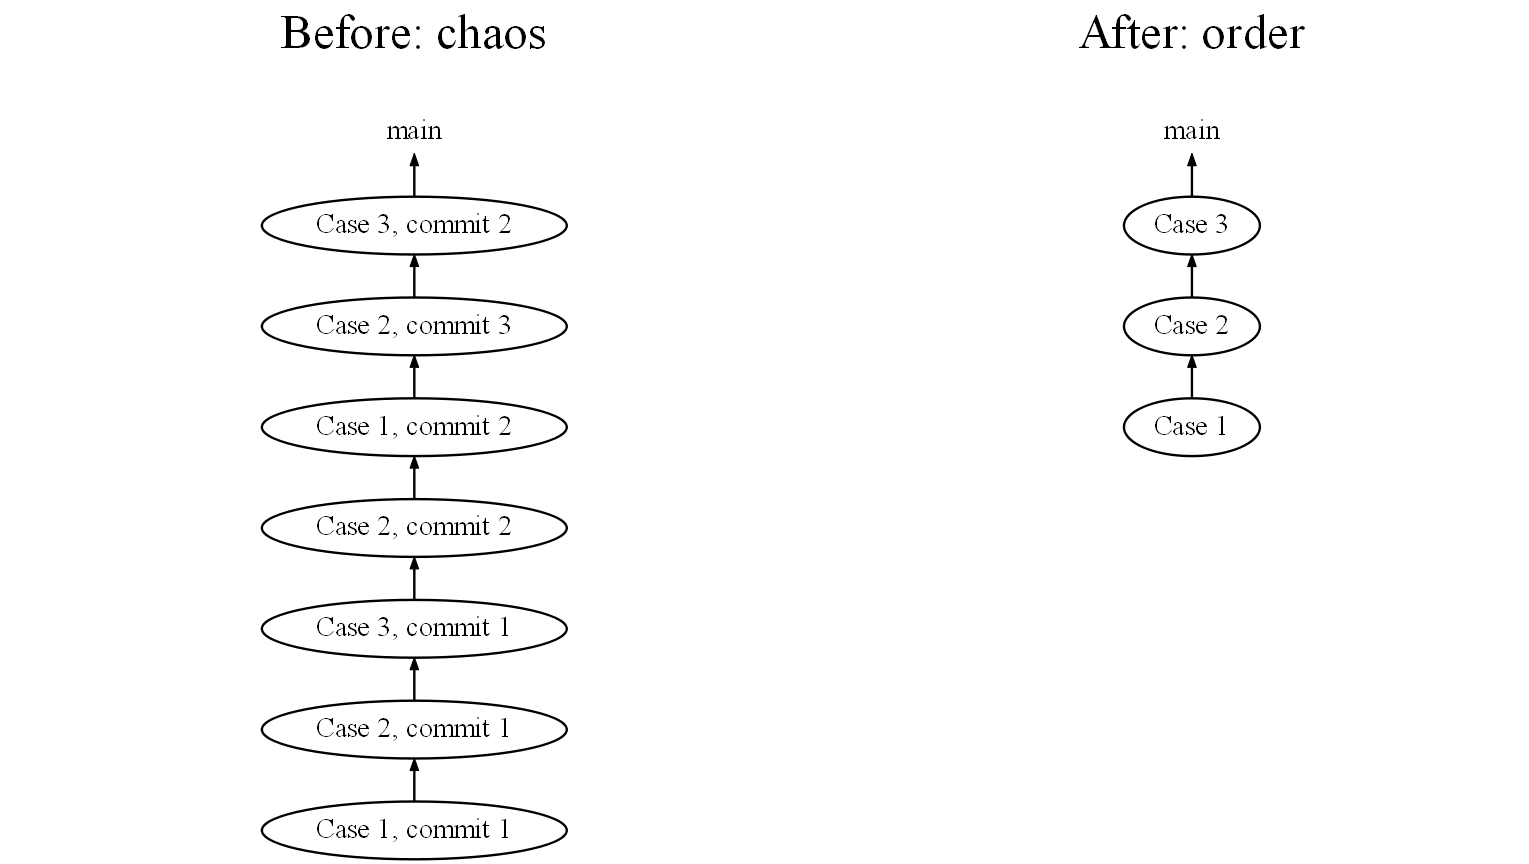
\includegraphics[scale=0.2]{02_2014_before-vs-after.png}
\end{figure}

\begin{thebibliography}{9}
\bibitem{Hlebnikov1} \url{http://thread.gmane.org/gmane.comp.version-control.git/189776}
\end{thebibliography}
\end{document}
